\documentclass{icmmcm}
%\usepackage[dvips]{graphicx}  % For importing graphics for use with
                              % dvips.
\usepackage[pdftex]{graphics} % For importing graphics for use with
                              % pdftex or pdflatex.
\usepackage[numbers]{natbib}

%%% Sample ICM/MCM Contest Submission
%%%
%%% C.M. Connelly <cmc@math.hmc.edu>
%%%   for the Department of Mathematics, Harvey Mudd College
%%%   Copyright 2003. 


%%% ---------------
%%% Local Command and Environment Definitions

%%% If you have any local command or environment definitions, put them
%%% here or in a separate style file that you load with \usepackage.

% \newtheorem declarations
\newtheorem{Theo1}{Theorem}
\newtheorem{Theo2}{Theorem}[section]
\newtheorem{Lemma}[Theo2]{Lemma}
% Each of the above defines a new theorem environment.
% Multiple theorems can be done in the same environment.
% Theo2's number is defined by the subsection it's in.
% Theo3 uses the same numbering counter and numbering system as
% Theo2 (that's the meaning of [Theo2]).


%%% TeX has an excellent hyphenation algorithm, but sometimes it
%%% gets confused and needs some help.
%%%
%%% For words that only occur once or twice, you can insert hints
%%% directly into your text, as in
%%%
%%%    our data\-base system is one of the most complex ever devised
%%%
%%% For words that you use a lot, and that seem to keep ending up at
%%% the end of a line, however, inserting the hints each time gets to
%%% be a drag.  You can use the \hyphenation command  to globally tell
%%% TeX where to hyphenate words it can't figure out on its own.

\hyphenation{white-space}

%%% End Local Command and Environment Definitions
%%% ---------------


%%% ---------------
%%% Title Block

\title{Conspirators Investigation}

%%% Which contest are you taking part in?  (Just one!)

\contest{ICM}

%%% The question you answered.  (Again, just the one.)

\question{C}

%%% Your Contest Team Control Number
\team{15118}


%%% A normal document would specify the author's name (and possibly
%%% their affiliation or other information) in an \author command.
%%% Because the ICM/MCM Contest rules specify that the names of the
%%% team members, their advisor, and their institution should not
%%% appear anywhere in the report, do *not* define an \author command.

%%% Defining the \date command is optional.  If you leave it blank,
%%% your document will include the date that the file is typeset, in
%%% the form  ``Month dd, yyyy''.

% \date{}

%%% End Title Block
%%% ---------------

\begin{document}

%%% ---------------
%%% Summary

\begin{summary}
  The contest rules specify that you should include a one-page summary
  of your report.  This page appears before the rest of the report,
  and will have a special header attached to it that takes up the top
  2.5" of the page.

  By typing your summary inside a \texttt{summary} environment, \TeX\ will
  handle the formatting of that page correctly, including leaving
  space at the top of the page and not numbering the page.
  
  It will also reset the page numbers so that the first page of your
  report is labeled correctly.
  
  What should you put here?  Basically, you want a brief restatement
  of the problem followed by a largely \emph{non-technical}
  description of what you've done.  Try to avoid using mathematical
  notation.
  
  You probably want to write a few paragraphs, around half to
  two-thirds of a page.

  For 2009, the COMAP folks said the following about the summary:
  \begin{quotation}
    The summary is a very important part of your MCM paper. The
    judges place considerable weight on the summary, and winning
    papers are sometimes distinguished from other papers based on
    the quality of the summary. To write a good summary, imagine
    that a reader may choose whether to read the body of the paper
    based on your summary. Thus, a summary should clearly describe
    your approach to the problem and, most prominently, what your
    most important conclusions were. The summary should inspire a
    reader to learn the details of your work.  Your concise
    presentation of the summary should inspire a reader to learn
    the details of your work. Summaries that are mere restatements
    of the contest problem, or are a cut-and-paste boilerplate
    from the Introduction are generally considered to be
    weak.

To Summarize:
\begin{description}
\item[Restatement Clarification of the Problem]
---

\item[Assumptions with Rationale/Justification]---emphasize those
  assumptions that bear on the problem. List clearly all variables
  used in your model.

\item[Model Design and justification for type model used/developed.]

\item[Model Testing and Sensitivity Analysis, including error
  analysis, etc.]

\item[Discuss strengths and weakness to your model or approach.]

\item[Provide algorithms] in words, figures, or flow charts (as a step
  by step algorithmic approach) for all computer codes developed.
\end{description}
 \citep{comap-mcm-rules}
\end{quotation}

\end{summary}
 
%%% End Summary
%%% ---------------

%%% ---------------
%%% Print Title Block, Contents, et al.

\maketitle
\tableofcontents

%%% Uncomment the following lines by deleting the % sign
%%% if you have figures or tables in your report:
\listoffigures
\listoftables  
 
%%% End Print Title Block, Contents, et al.
%%% ---------------

\section{Introduction}%
\label{sec:introduction}


Our organization, the Intergalactic Crime Modelers (ICM) is working
for a criminal case of a bank company.  
There are indications that there is a conspiracy within the company. 
It is believed that the conspirators want to embezzle funds from
the company and to steal funds from credit card 
Careful logs have been kept of whom has sent messages related to each
topic and whom received these messages.

The goal to approach this problem is to determine a priority list, 
to draw a discriminate line, and if possible to find
conspiracy leaders. In addition, we also want to use semantic
network analysis to improve the result and examine applications of
our developed techniques in other fields such as diseased biology.

\noindent -------------------- TODO:
the history and context of the problem,
and your work and results.  Your introduction should be more detailed
and technical than your summary.  You may also want to include an
outline of your report, along the lines of
\begin{quotation}
  In Section~1 we give our definitions and notation. Section~2
  describes our numerical experiments\ldots{}..
  
  We prove our main result, Theorem~6, in Section~5\ldots{}.
\end{quotation}
Of course you would replace the numbers in that example with
appropriate \verb|\ref| commands pointing to the correct
\verb|\label|s in your source.\\
-----------------------

\section{Given Information}
\begin{enumerate}
\item We are given that Jean, Alex, Elsie, Paul, Ulf, Yao,
and Harvey are conspirators.
\item We are given that Darlene, Tran, Jia, Ellin, Gard, Chris,
Paige, and Este are \textit{not} conspirators.
\item There are 83 nodes, 400 links, and 15 considered topics.
\item Topics 7, 11, and 13 are known to be suspicious topics.
\end{enumerate}

\section{Assumptions}

\begin{enumerate}
\item Assume that it is unlikely that conspirators communicate
conspiratorial topics to non-conspirators.
\end{enumerate}
\section{Methodology: Model Design and Model Algorithms}

The algorithm works primarily by giving a different weight to each of the 
topics based on who is in the conversation. We will run the algorithm
a couple of times to adjust the likelihood of being conspirators
based on the new information gained from the most 
recent round of analysis.

\subsection{Setting Up}
In this model, we define the following parameters:
\begin{enumerate}
\item  For each person $i$ where $i=0,1,2,\ldots, 82$, 
we the probability (``certainty'')
that each person is a conspirator, $c_i,$
where $0\leq c_i \leq 1.$ 
If $c_i=1$, for example, it means that the person
with number $i$ has $100\%$ chance to be
a conspirator, according to our model. 

\item  For each person $i$ where $i=0,1,2,\ldots, 82$, in each round of running,
we give that person a score $s_i$. High score indicates
the likelihood to be a conspirator, based on the set
of probability of people being conspirators from each round.
The difference in the score $s_i$ and the probability $c_i$ of
being a conspirator is that the score $s_i$ is calculated in each round
and will affect the probability $c_i$ in the end of each round
based on the ranking of the score, whereas $c_i$ is the long-run
probability that will eventually indicate a priority list and
a discriminate line.

\item For each topic $j$ where $j=1,2,\ldots,15,$
we give a weight $w_j$ where $0\leq w_j\leq 1.$
The more weight of the topic has, the more suspicious it is.

\item  We assign the involvement of person $i$ to the topic $j$ the number
$\alpha_{i,j}.$
\end{enumerate}

Note that we use python to model the problem.

\subsection{Initializing}
\begin{enumerate}
\item To initialize the values, we set $c_i = 1$ for those that
we know to be not conspirators ($i=18,21,7,54,67,49$)
and we set $c_i = 0$ for those that
we know \textit{not} to be conspirators ($i=48,64,65,68,74,0,2,7$).
Otherwise, we set $c_i = 0.5.$ In short, in the initial states
\[c_i=
\begin{cases}
1,	& \text{person $i$ is known to be a conspirator}\\
0,	& \text{person $i$ is known \textit{not} to be a conspirator}\\
0.5,	&\text{otherwise.}
\end{cases}\]

\item To calculate $s_i,$ we use the following formula,
which is the weighted sum of the involvement in each topic,
\[s_i = \sum_{j=1}^{15} \alpha_{i,j} w_j.\]

\item We rank each person based on the score.
The group of people who are likely to be 
cons
\end{enumerate}

\subsection{Recalculating}
\begin{enumerate}

\item Run the programs a couple of times to recalculate
the score 

\item For each person $i$,
if he or she has a 
rank higher than that of the lowest-score known conspirators less a constant,
we adjust his or her certainty (probability) by the following scheme:
\[c_i := \frac{1 + c_i}{2}.\]
That is, we take the average with 1 and replace the original by the new value. 
Because the original $c_i$ is less than 1, the net effect is that
$c_i$ will be increased so that it is closer to 1 by half-distance.

\item Similarly,
for each person $i$,
if he or she has a 
rank lower than the highest-score known non-conspirators plus a constant,
we adjust his or her certainty (probability) by the following scheme:
\[c_i := \frac{c_i}{2}.\]
That is, we take the average with 0 and replace the original by the new value. 
Because the original $c_i$ is greater than 0, the net effect is that
$c_i$ will be decreased so that it is closer to 0 by half-distance.

\end{enumerate}
\section{Theorems}
\begin{Theo1}
The algorithm converges.
\end{Theo1}
{\bf Proof.}
The idea might be because we take the average with 1 the 
probability of people who have
ranks higher than that of the lowest-score known conspirators less a constant, and we
take the average with 0 the 
probability of people who have ranks lower than the highest-score known non-conspirators plus a constant.
The list of the people in those two groups should not overlap,
so we will not take the average with 0 and 1 alternatively.
By using the sum of constants or some multiplication factor
those two lists should keep expanding until they meet.
Everyone should be absorbed by exactly one group. 
\hfill $\Box$

%%=================NEW SECTION
\section{Model Testing}

Here is the result (sure we need to clean this up):


[('Yao', 269.3696826414443), ('Alex', 248.25159624805804), ('Ulf', 170.44607292282194), ('Elsie', 107.91782710259969), ('Seeni', 69.4092311734181), ('Marion', 60.15081667708738), ('Jerome', 59.913589798879265), ('Harvey', 55.84169703322986), ('Paul', 54.90632647134443), ('Jean', 40.77878818732485), ('Dolores', 32.159531342553116), ('Kim', 24.361643919169694), ('Gretchen', 23.367079384713396), ('Sheng', 21.46496497943977), ('Cha', 21.32613685445123), ('Dwight', 20.223057774180393), ('Dayi', 16.42221253399016), ('Bariol', 9.562466862329252), ('Fanti', 9.057530816272097), ('Christina', 8.049446869004532), ('Jia', 7.114818405452967), ('Phille', 1.9477975402344825), ('Lars', -0.2836634825684179), ('Andra', -2.000893947500348), ('Wayne', -4.023420759543937), ('Donald', -4.488572562295921), ('Paige', -5.225896391287632), ('Priscilla', -6.477615906899372), ('Carina', -7.284821427828006), ('Chara', -8.980050446822759), ('Neal', -9.15908188762064), ('Cole', -9.161113660274463), ('Vind', -9.37641612827602), ('Lao', -10.638792965330348), ('Darol', -10.638792965330348), ('Quan', -10.777621090318888), ('Tran', -10.777621090318888), ('Melia', -10.97657110161257), ('Elsie', -11.159866202827182), ('Este', -11.707899437878071), ('Le', -12.892255434070426), ('Beth', -14.000335170803277), ('William', -14.451848008330307), ('Olina', -14.810490114752707), ('Malcolm', -15.95065658409456), ('Gard', -16.775782982369233), ('Patricia', -17.403657335757607), ('Marcia', -17.77818082892289), ('Douglas', -18.297595195522916), ('Eric', -18.527678829306797), ('Han', -18.620969465676513), ('Patrick', -18.968384621380654), ('Wesley', -19.217712858040336), ('Louis', -19.73806188412489), ('Mai', -20.136926656651013), ('Reni', -25.044747025310144), ('Gerry', -27.84161523651497), ('Neal', -28.138771651542996), ('Karen', -28.24143810389287), ('Katherine', -28.674060454652754), ('Kristine', -28.786657180218235), ('Erica', -30.459336719804245), ('Hazel', -30.518251825693312), ('Crystal', -31.074338419707306), ('Cory', -32.830990184663776), ('Darlene', -33.93175600242964), ('Hark', -34.93254144093831), ('Ellin', -37.89102658270057), ('Chris', -38.914488351308634), ('Sherri', -41.2563817419928), ('Shelley', -42.464974881047794), ('Sandy', -46.55155420242029), ('Francis', -48.33271922878934), ('Lois', -51.404305327685584), ('Julia', -65.35422875982475), ('Stephanie', -65.3999527056968), ('Jerome', -72.62795945161139), ('Gretchen', -82.17572060966768), ('Claire', -84.77047848286455), ('Beth', -87.44729613327095), ('Kristina', -93.41477879711616), ('Marian', -94.83303782341783), ('Franklin', -103.68927258753226)]
Certain = [0, 0, 0.75, 0.75, 0, 0, 0, 1.0, 0, 0, 0.875, 0, 0, 0.9999999999854481, 0, 0, 0.9999999999708962, 0.5, 1.0, 0, 0, 1.0, 0, 0, 0, 0, 0, 0, 0, 0, 0, 0, 0.5, 0, 0, 0, 0, 0, 0, 0, 0, 0, 0, 1.0, 0, 0, 0, 0, 0, 1.0, 0, 0, 0, 0, 1.0, 0, 0, 0, 0, 0, 0, 0, 0, 0, 0, 0, 0, 1.0, 0, 0, 0, 0, 0, 0, 0, 0, 0, 0, 0, 0, 0, 0.9999999999708962, 0]
Uncertain = [1.0, 0.9999999999990905, 1.0, 0.999999999992724, 0.875, 0.9999999999990905, 0.9999999999990905, 0, 0.9999999999990905, 0.9999999999990905, 0.5, 0.9999999999990905, 0.9999999999990905, 0.75, 0.9999999999990905, 0.9999999999990905, 0.875, 0.9999999999990905, 0, 0.9999999999990905, 0.9999999999990905, 0, 0.9999999999990905, 0.9999999999990905, 0.9999999999990905, 0.9999999999990905, 0.9999999999990905, 0.9999999999990905, 0.984375, 0.9999999962747097, 0.9999999999990905, 0.9999999999990905, 0.9999999999990905, 0.9921875, 0.9999999999990905, 0.9999999999990905, 0.9999999999990905, 0.9999999999990905, 0.9999999999990905, 0.9999999999990905, 0.9999999999990905, 0.9999999997671694, 0.9999999999990905, 0, 0.9999999999990905, 0.9999999999990905, 0.9999999999990905, 0.998046875, 1.0, 0.75, 0.9999999999990905, 0.9990234375, 0.9999999999990905, 0.9999999999990905, 0, 0.9999999999990905, 0.998046875, 0.998046875, 0.9999999999990905, 0.9999999999990905, 0.9999998807907104, 0.9999999999990905, 0.9999999999990905, 0.9999999999990905, 1.0, 0.9998779296875, 0.9999999999990905, 0, 1.0, 0.9999999999990905, 0.9999999999990905, 0.9999999999990905, 0.9999999962747097, 0.9999999999990905, 1.0, 0.9998779296875, 0.9999999999990905, 0.9999999999990905, 1.0, 0.9999990463256836, 0.9998779296875, 0.875, 0.9999999999990905]

		We need to fix somehow though, to make certain + uncertain = 1.
		(Maybe we can go back to when we have only one list, so that we can
		always impose this condition)
%Take a look at an example below, where we put the city into our hexagonal coordinate (Both X and Y range from -3 to 3):
%\begin{table}[htbp]
%  \begin{center}
%    \begin{tabular}{@{}c|rrrrrrr@{}} \toprule
%X and Y  	&-3 	&-2 		&-1		&0		&1		&2		&3\\ \midrule   
%3&15.53	&34.87	&36.03	&32.00	&0.00	&0.00	&0.00    \\ 
%2&36.73	&76.12	&104.57	&81.22	&43.00	&0.00	&0.00	\\
%1&37.13	&94.27	&137.75	&138.05	&91.57	&54.00	&0.00	\\
%0&31.0	&82.1	&134.47	&\textbf{158.42}	&140.13	&83.07	&35.00	\\
%-1&0.00	&51.0	&113.25	&137.35	&145.05	&111.92	&39.12	\\
%-2&0.00	&0.00	&49.00	&89.37	&99.00	&92.42	&46.47	\\
%-3&0.00	&0.00	&0.00	&33.00	&32.15	&36.18	&27.72	\\
% \bottomrule	
%    \end{tabular}
%  \end{center}
%  \caption[A Distribution of Repeaters for a Uniform Distribution of People]{The table of the number of conversations (reflecting the number of repeaters) at each point. The number of people is 1000. The level of hexagons is 3.}
%  \label{tab:uniform}
%\end{table}
%
%From Table~\ref{tab:uniform}, we have the total number of repeaters of 2,780. Hence, the actual number of repeaters needed (with help of PL tones) is 51.48. As there are $6\times(3^2)=54$ regions as well, the number of repeaters needed per 1 PL tone per 1 location is 0.953. This can be done easily since we have 3 frequency sets to serve. One concern is the service at the peak: the middle (point $(0,0)$). The original number of repeaters needed is 158.42. By using PL tones, we have the avearge of $2.93$ users using one PL tone. Again, this use can be accommadated by 3 different sets of frequencies. Thus, in this case, the total number of repeaters required is 51.48, approximately \boxed{52 \text{ repeaters}} , each holding differnt 54 PL tones.

%Figure~\ref{sample1} is an example of repeater coordination.
%\begin{figure}[!hbtp]
%\makebox[\textwidth]{\framebox[8cm]{\rule{0pt}{8cm}}}
%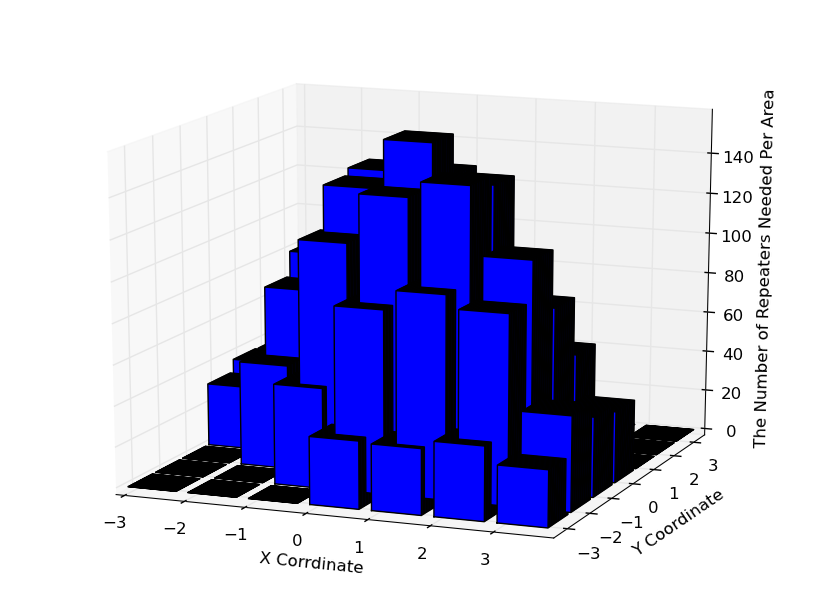
\includegraphics[width=7cm]{sample1.png}
%\caption{Sample 1 Distribution of Repeaters (Maximum at the Middle).\label{white}}
%\end{figure}

%Figure~\ref{fig:sample1} is an example of repeater coordination.
%\begin{figure}[ht]
%\begin{center}
%\scalebox{0.6}{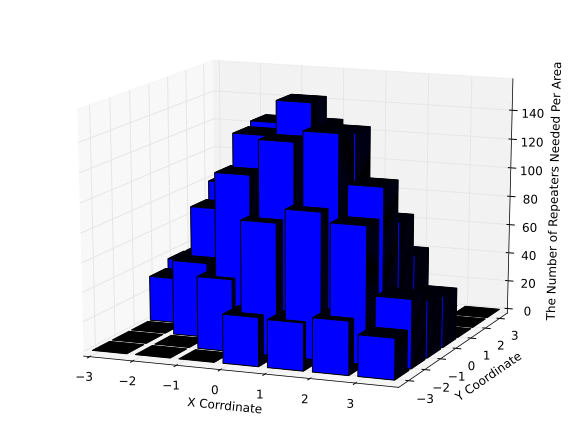
\includegraphics{sample1}}
%\end{center}
%\caption[A Distribution of Repeaters for a Uniform People Distribution]{A Distribution of Repeaters (Maximum at the Middle).\label{sample1}}%
%\label{fig:sample1}
%\end{figure}

\section{Sensitivity Analysis And Error Analysis}
Idea: change the input. Say what if we know that someone is a conspirator
or someone has a higher chance than $0.5,$
how much the result will change.
\section{Strengths and Weaknesses}

\section{Possible Improvements}
\begin{enumerate}
\item We need to come up with an indicator of how good our results are.
Like testing hypothesis. Suppose the conspirator groups are 
like what we have. [[[From here, it might be a good idea to go back
and explain that it is not plausible to do exhausive search of
$2^{83}$ possibilities.]]]
\item Add the ability to adjust the number of people to do penalty: int(original/k), varying k.
\item Consider the bosses (Jerome, Delores, Gretchen) more carefully.
\item Keep the level of suspiciousness for 7, 11, 13 (or at least see how those change)
\item Implement semantic network analysis. 
	Or even now we notice some spanish stuff in more than one topic discussion
	so we can maybe group the topic or somehow tie the scores of those topics together
\item Think about the relationship to other fields: infected, diseased cells in a bio network
\end{enumerate}
		

\section{Conclusion}

All's well that ends well.


%%% ---------------
%%% Bibliography

%\nocite{*}   %%% Include everything in the thesis.bib file.  Be
             %%% careful---some journals and fields expect you to only
             %%% include references for materials that you have
             %%% actually cited in your paper, others allow you to
             %%% include materials you used as ``background'' without
             %%% actually citing specific pages or passages.

%%% Feel free to choose any bibliography style you like.
\bibliographystyle{plainnat}
%%% The filename (without the bib extension) of your bibliography file.
\bibliography{icmmcm}

\end{document}



